\begin{enumerate}
\item \runningj \nonet ในการเคลื่อนที่เป็นเส้นตรง  กราฟข้อใดแสดงว่าวัตถุเคลื่อนที่ด้วยความเร็วคงตัว
	\begin{4c}
		{\begin{adjustbox}{valign=t}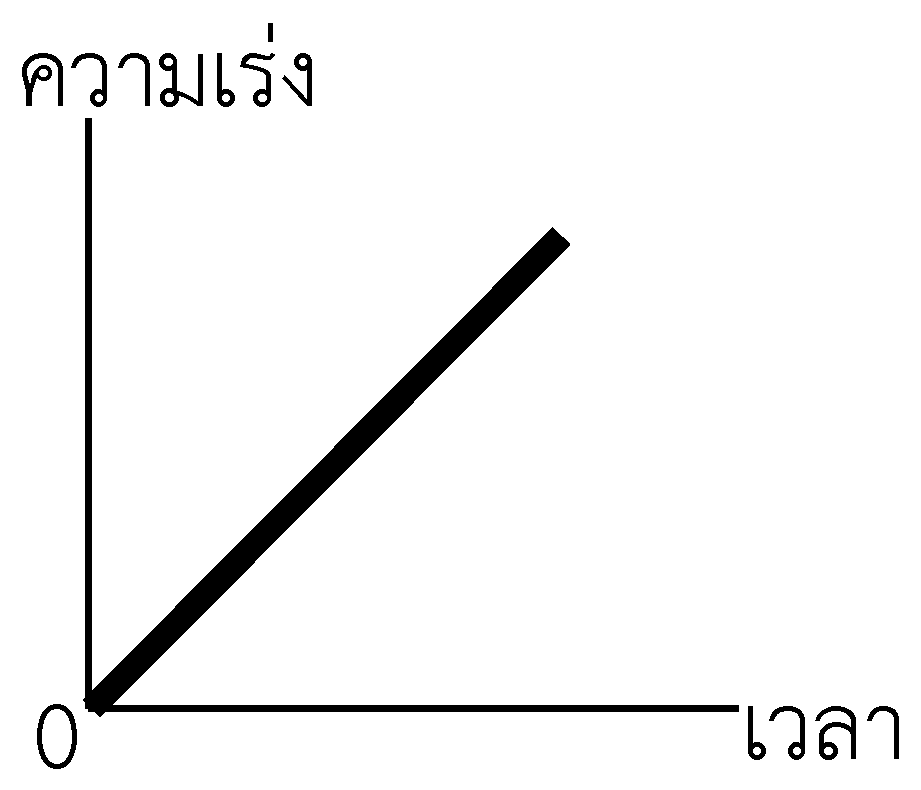
\includegraphics[width=\linewidth]{pic-17-1.pdf}\end{adjustbox}}
		{\begin{adjustbox}{valign=t}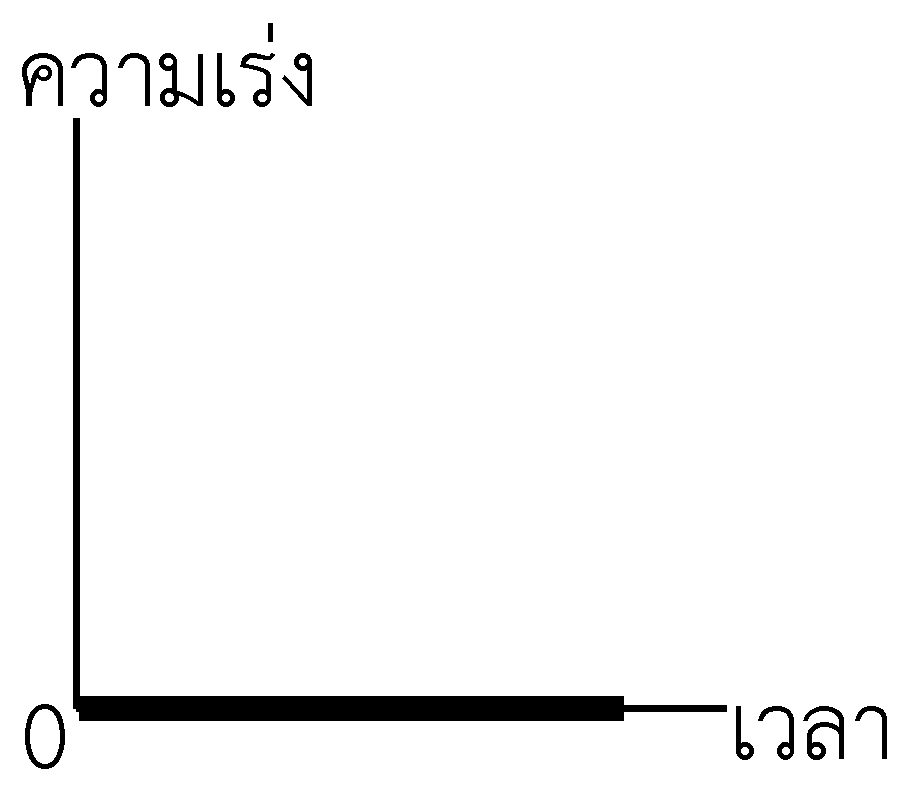
\includegraphics[width=\linewidth]{pic-17-2.pdf}\end{adjustbox}}
		{\begin{adjustbox}{valign=t}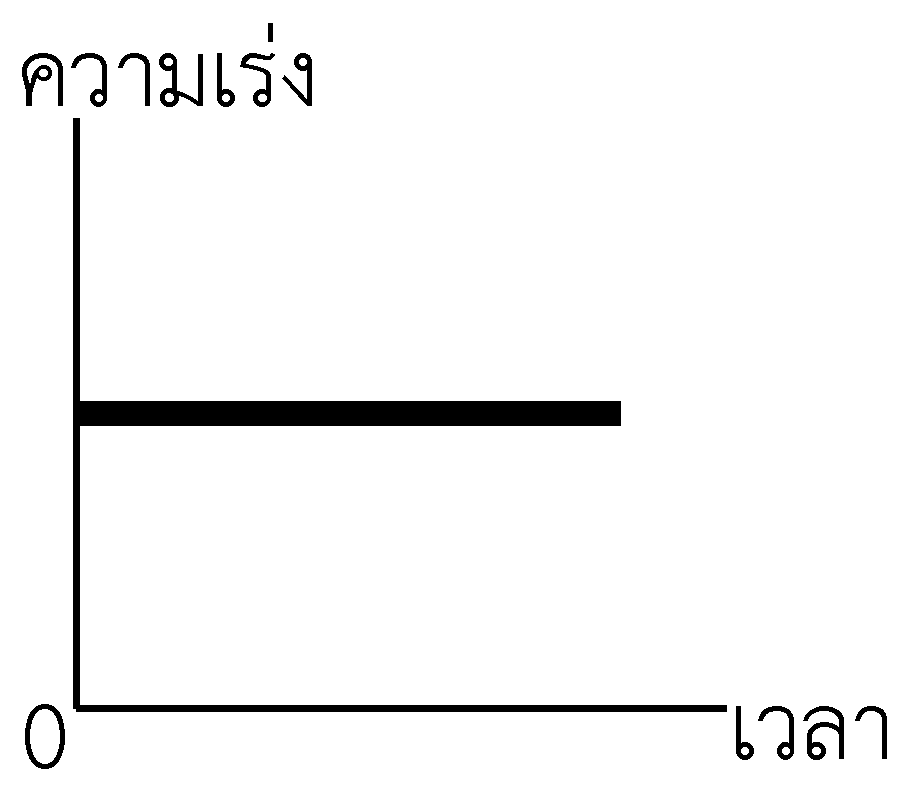
\includegraphics[width=\linewidth]{pic-17-3.pdf}\end{adjustbox}}
		{\begin{adjustbox}{valign=t}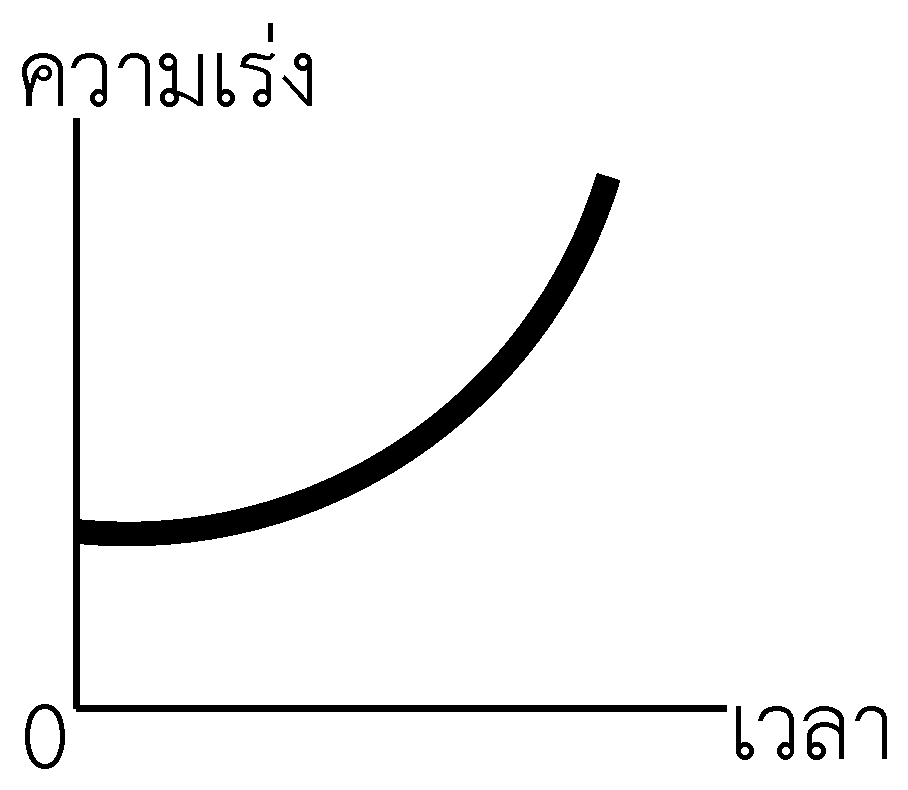
\includegraphics[width=\linewidth]{pic-17-4.pdf}\end{adjustbox}}
	\end{4c} 
\end{enumerate}
